\documentclass[12pt,titlepage]{report}
\usepackage{graphicx}
\usepackage{hyperref}
\hypersetup{colorlinks=true}
\begin{document}
\title{\Huge{Argus} 
\\  \large\emph{User Manual}}
\author{Matthew Crispin Scicluna}
\maketitle
\pagebreak
\tableofcontents
\chapter{Introduction}
\section{What is Argus?}
Argus is a computer program written in the programming language R. It was written by Matthew Scicluna from June 2013 to January 2014. Argus' main purpose is to convert the raw output from an existing program called theRealFishTracker into meaningful statistics that can be interpreted by Psychologists and Biologists. To begin using Argus, one must have R installed on their computer and must open an R file called switchboard. The switchboard is where you input all of your parameters and choose which functions to run.
\paragraph{What is a Function?}
I will give a simple definition of what a function is here so the reader may be able to follow me along during later chapters. A function is basically a set of commands that may or may not require user input to produce useful statistics for the user. Essentially we are asking the computer to interpret the data in some specific way. An example of a function would be the first function I wrote for this program, which is the speed function. This function takes no parameters but will tell the user how fast the fish travelled in during the duration of the trail, measured in cm/sec.

\section{What is theRealFishTracker?}
This program utilizes a previously created program called theRealFishTracker, built by James McCrae in 2011. A good description of the program and its download information can be found at \url{http://www.dgp.toronto.edu/~mccrae/projects/FishTracker/}. The program converts a video file into a text document. The output can be analyzed using theRealFishTracker itself, but the programs own analysis is suboptimal for the kinds of large scale data sets expected in modern psychological and biological research.The raw text file can instead be read into Argus. Perhaps we are getting ahead of ourselves; before any analysis can occur we must first install Argus.
\begin{figure}[ht!]
\centering
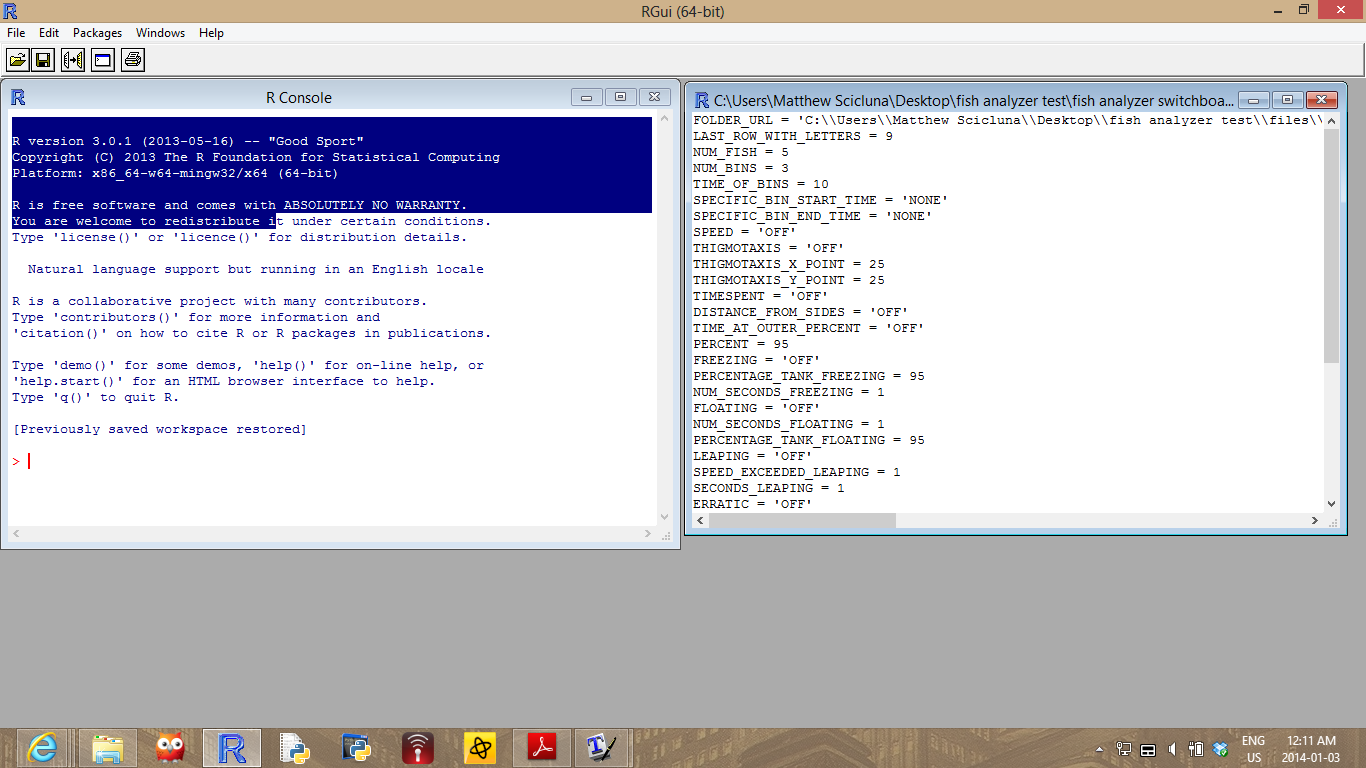
\includegraphics[width=120mm]{image1.png}
\caption{Switchboard open in R's GUI}
\label{overflow}
\end{figure}


\chapter{Startup}
\section{Installing Argus}
Before continuing, you will have to install R and the packages \texttt{xlsxjars} and \texttt{rjava}. More information about R can be found online at \url{http://cran.r-project.org/}
 Argus consists of 4 files: the text documents \emph{fish analyzer program}, \emph{multi case fish analyzer program} and \emph{cutoff times (in seconds)} and the R file \emph{fish analyzer switchboard}. These are to be put inside of a folder called Argus (or whatever you choose to name it). Also, inside this new folder is to be another folder where the text files from theRealFishTracker are to be stored. This new folder will hold the files to be analyzed by Argus.
To begin running Argus, place the text file output from theRealFishTracker into the folder mentioned above. This program can hold however many output files from theRealFishTracker as you want, and will analyze them all simulteneously. \\
\paragraph{A Note About What Not to Do}
Be mindful of the similarities between files that you put into the folder in this program. If you desire a uniform number of time bins, then you should not put files with significantly varying times, unless you strickly specify the number and time of each bin (more on this in chapter 3). \\
\section{Setting Cutoff Times}
Once you have the selected files in the folder, go to the text file \emph{Cutoff Times (in seconds)}. Next to a marvelous drawing of a Zebrafish (drawn by yours truly) there is a single line that reads:
\begin{verbatim}
CUTOFF_TIMES_LIST = c(0, ... ,0)
\end{verbatim}

replace this with a list of numbers where each number represents the amount of time (in seconds) that you wish to remove from the beginning of the trial. So, for example, I have two files in the folder, and I want to remove 30 seconds from the second file  and 10 seconds from the first, then I would replace the list of 0's with:
\begin{verbatim}
CUTOFF_TIMES_LIST = c(10, 30)
\end{verbatim}
You can add or remove any number of entries from this list until it has the same number of entries as there are files in the folder you are intending on analyzing. If you do not wish to remove any time from a particular file, just leave the default entry of 0 in the list.
Now load the R file \emph{ fish analyzer switchboard.R}. This can be done easily by loading R itself, going to \texttt{file} clicking \texttt{open script}, and selecting \texttt{ fish analyzer switchboard.R}
\begin{figure}[ht!]
\centering
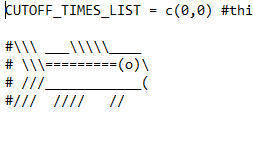
\includegraphics[width=50mm]{image2.png}
\caption{\emph{Cutoff Times in Seconds} file}
\label{overflow}
\end{figure}

\pagebreak
\section{The Switchboard}
The switchboard is the main user interface of the program. It appears next to R's console (the screen that opens by default when you load R)
\begin{figure}[ht!]
\centering
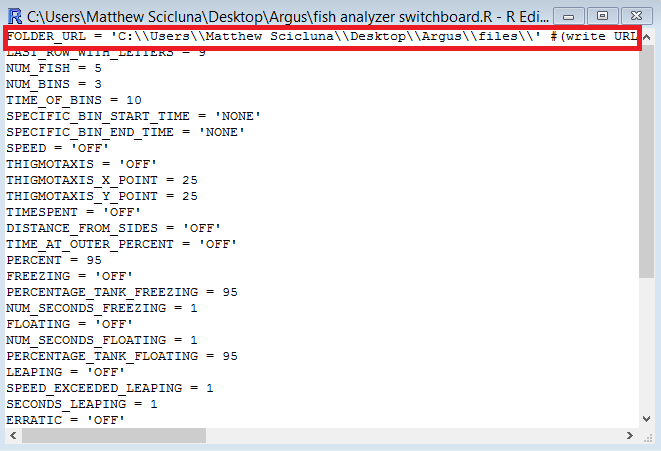
\includegraphics[width=120mm]{image6.png}
\caption{where the directory is on the switchboard}
\label{overflow}
\end{figure}

Change this directory to the directory of the folder containing the files to be analyzed. The directory is to be put in the line marked by a red box in the image above, by default it is set to
\begin{verbatim}
FOLDER_URL = 'C:\\Users\\Matthew Scicluna\\Desktop\\Argus\\files\\'
\end{verbatim}
Once this is done you can begin modifying the switchboard so that you get the precise output that you want. This will be the main focus of the next chapter.
Before we begin tinkering with the switchboard, there are more things to bear in mind. Firstly, scroll down the switchboard until you get to the following lines (marked in a red box in Figure 2.3). Ensure that these referring to the correct files, and that the directory is correct for all of them. 
\paragraph{Useful trick} An easy way to obtain the directory is to simply to drag and drop the files from their folder into R's command line and then R will display the directory with an error message. One can simply copy the directory from here. \\

The line below this asks for the specific number of lines that are to be removed from the text files. Typically the output from theRealFishTracker has 7 or 9 lines before the lines with actual fish coordinates. These lines are important and should not be removed pre-analysis, but must be internally ignored by the program during most of its execution. What you must do is check the text file for the last line that doesn't have fish coordinates on it (line 7 in Figure 2.4, for example).
The line below that asks for the number of fish which is in your trial. Note that there are different functions you are allowed to run if you have one fish versus multiple fish.
\paragraph{Final Note} Recall earlier I mentioned that you needed to bear in mind what kind of files would be suitable for simulteneous analysis (which files should be read together in the same folder). Notice that the values entered into the switchboard is the same for each file being simulteneously analyzed. This means that if, for example, if one trial has 4 fish in it and another has 2, then they should not be analyzed simulteneously, as there is no way to tell the program \emph{ 'trial A has 4 fish but trial B has only 2'}.

\section{Bin Specifications}
The next 4 lines in the switchboard read:
\begin{verbatim}
NUM_BINS = ...
TIME_OF_BINS = ...
SPECIFIC_BIN_START_TIME = ...                                  
SPECIFIC_BIN_END_TIME = ...                                 
\end{verbatim}
It is here where you can specify the number of bins you want the program to make, the time of each bin (in seconds), or both (in case you want a specific number of bins that are each of a particular length. If you only want one bin, then you have the flexibility to have it begin and end \emph{precisely} wherever you want within the video file, this is done by specifying the \texttt{SPECIFIC BIN START TIME} and \texttt{SPECIFIC BIN END TIME}. If you do not need to specify any of these parameters (an example would be if you want 1 minute bins but dont care how many bins you would get), than you would set time of bins to  \texttt{60} and number of bins to \texttt{'NONE'} --- this doesn't mean that you want to get no bins, but rather that you are not specifying any specific amount of bins to be created. 

\begin{figure}[ht!]
\centering
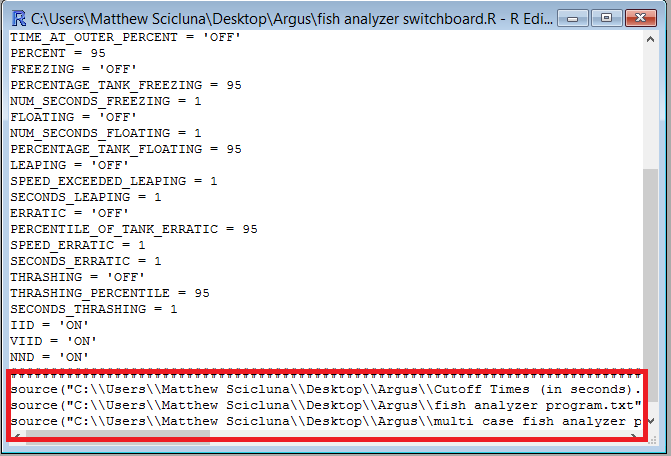
\includegraphics[width=100mm]{image3.png}
\caption{you should check the directory of these files also}
\label{overflow}
\end{figure}

\begin{figure}[ht!]
\centering
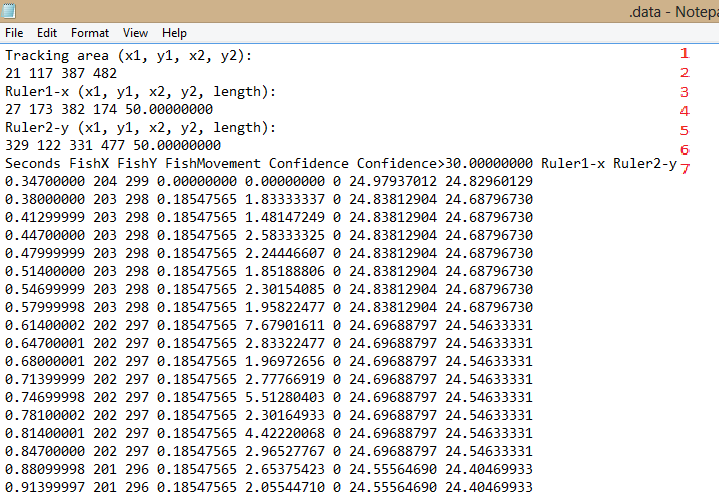
\includegraphics[width=100mm]{image8.png}
\caption{what lines to be removed from the text file}
\label{overflow}
\end{figure}

\chapter{Functions}
Now that you have specified the directory of the folder, the number of fish and kinds of time bins you want; you are ready to specify the kind of information you want Argus to extract from the raw text files generated from theRealFishTracker. The remaining lines in the switchboard are all either functions or parameters of the functions. Earlier we defined what a function was, now we will define what a parameter is.
\section{What is a Parameter?}
A parameter is a value that is associated with a function. Changing the value of the parameter may change the value of the output statistic of the function. An example of this is the Thigmotaxis function. The thigmotaxis function produces a statistic which is the average distance the fish was from some point in the fish tank. This point is specified by an x and y coordinate, which are the functions 2 parameters. It can be seen that a changing the parameter (and thus specifying a new point) will affect the statistic, as it is now measuring the average distance of a fish to a \emph{different} point. 
\section{Functions for Single Fish Trials}
Functions in Argus only either work for trials with tracking of a single fish, or with trials with tracking of multiple fish. These are the functions that work only for analyzing trials where one fish was tracked. These functions will not work if you use them in trials where multiple fish were tracked at once. To turn on a function, next the the function name, replace \texttt{FUNCTION NAME = 'OFF'} with \texttt{FUNCTION NAME = 'ON'}.
\subsection{SPEED}
Calculates speed, acceleration, distance travelled and fastest speed of the fish during each time bin.
\subsection{THIGMOTAXIS}
Average distance from fish to a point in the fishtank specfied by the parameters \texttt{THIGMOTAXIS X POINT} and \texttt{THIGMOTAXIS Y POINT}. 
\subsection{TIMESPENT}
Calculates the time fish spent accelerating, changing direction, staying still, and moving at particular speeds during each time bin.
\subsection{DISTANCE FROM SIDES}
Calculates the average distance the fish was to each side and to the top and bottom of the fish tank during the duration of each time bin.
\subsection{TIME AT OUTER PERCENT}
Calculates the time the fish spent in the periphery of the fishtank. The periphery is specified by the parameter \texttt{PERCENT}, which represents the inner percentile of the fishtank for which this function calculates the time the fish was away from.
\subsection{FREEZING}
Number of times fish was detected freezing. The parameters are: 
\begin{itemize}
\item \texttt{PERCENTAGE TANK FREEZING}: The outer periphery the fish must be in for freezing to be considered happening and \item \texttt{NUM SECONDS FREEZING}: The number of seconds fish performs freezing activity for program to consider it freezing.
\end{itemize}
\subsection{FLOATING}
Number of times fish was detected floating. The parameters are: 
\begin{itemize}
\item \texttt{NUM SECONDS FLOATING}: the number of seconds fish performs floating activity for floating to be considered to have happened 
\item \texttt{PERCENTAGE TANK FLOATING}, the outer percentile of tank fish need to be \emph{in} for duration of behavior for it to be considered for floating.                                                      
\end{itemize}
\subsection{LEAPING}
Number of times fish was detected leaping. Parameters are: 
\begin{itemize}
\item \texttt{SPEED EXCEEDED LEAPING}, the minimum speed fish must maintain during leaping behavior for program to recognize behavior
\item \texttt{SECONDS LEAPING}, the number of seconds fish performs leaping activity for program to consider it leaping.
\end{itemize}
\subsection{ERRATIC}
Number of times fish was detected having erratic behavior. Parameters are: 
\begin{itemize}
\item \texttt{PERCENTILE OF TANK ERRATIC}, the outer percentile of tank fish needs to be in for behavior to be considered erratic \item \texttt{SPEED ERRATIC}, minimum speed fish must maintain during erratic behavior for program to recognize behavior
\item \texttt{SECONDS ERRATIC}, number of seconds fish performs erratic activity for program to consider it erratic.
\end{itemize}
\subsection{THRASHING}
Number of times fish was detected thrashing. Parameters are: 
\begin{itemize}
\item \texttt{THRASHING PERCENTILE}: percentile of tank fish must be swimming outside of for behavior to be considered thrashing. \item \texttt{SECONDS THRASHING}: number of seconds fish performs thrashing activity for program to recognize behavior.
\end{itemize}
\section{Functions for Multiple Fish Trials}
If you have trials where multiple fish are being tracked at once, and you've set \texttt{NUM FISH}  to be greater than 1, then you cannot use the abovementioned functions. There are three functions you can use, however.
\subsection{IID}
\emph{Inter Individual Distance}: The average distance from each fish to each of the other fish. This function will produce this statistic for each fish tracked. So if there are 3 fish in your trial, this function will generate the average of the average distances from fish 1 and 2; and fish 1 and 3. These values will appear in the printout in adjacent rows.
\subsection{VIID}
\emph{Variance of Inter Individual Distance}: The variance between the average distance between each fish and each other fish. Also produces a value for each fish being tracked in each trial.
\subsection{NND}
\emph{Nearest Neighbour Distance}: The distance from each fish to its "nearest neighbour" --- the fish that was physically closest to it during the duration of each time bin. Produces a statistic for each fish.
\ 
\chapter{Output}
In this chapter we will discuss the final output of the program and what you can do with it. Once you have selected all the functions and parameters you want, click the switchboard and then go to \texttt{Edit}, then click \texttt{Run all}. The program will execute, taking a few minutes to run. Once it is finished running you will get a notification. You will find the output file named \texttt{output. excelfile} in the same folder where the raw files from theRealFishTracker are. A typical output file will look like Figure 4.1:

\begin{figure}[ht!]
\centering
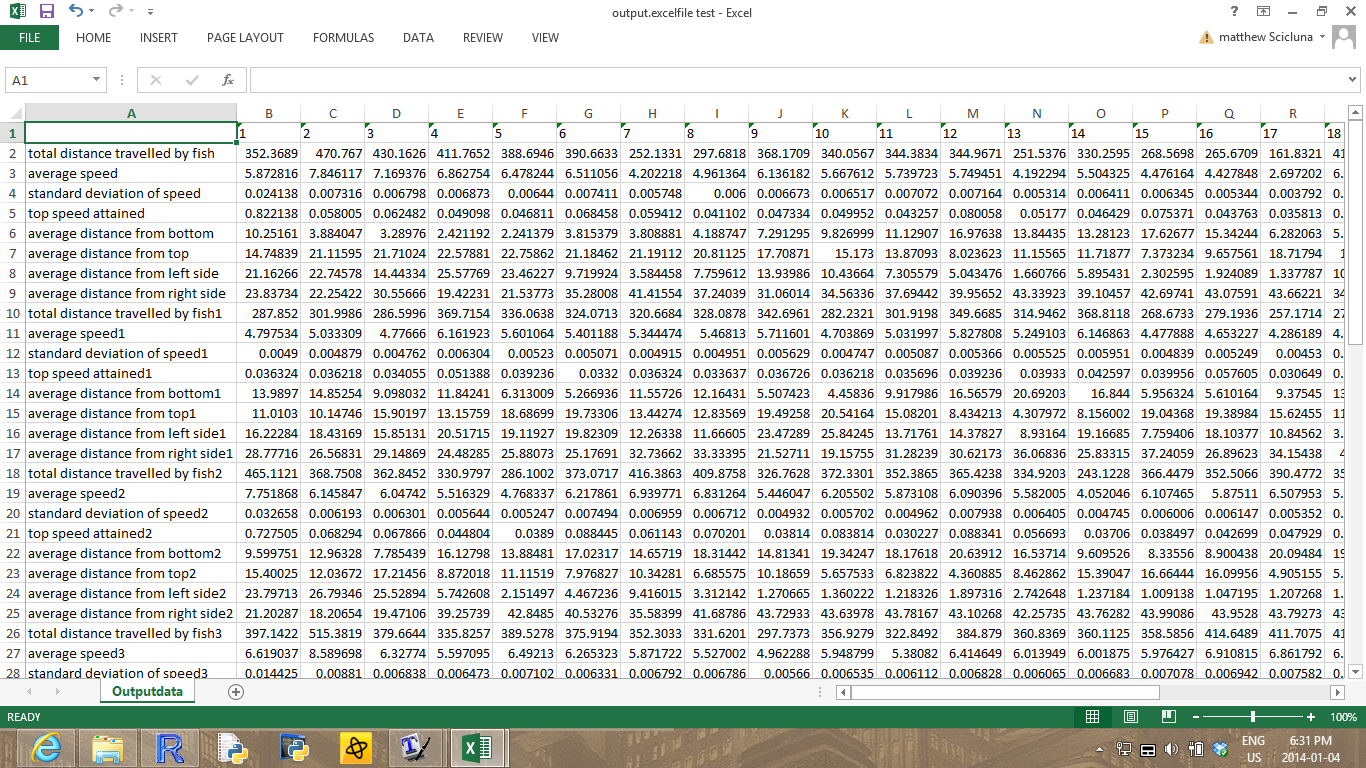
\includegraphics[width=120mm]{image10.png}
\caption{Typical Output From Argus}
\label{overflow}
\end{figure}
\pagebreak
\section{Navigating the Output File}
Notice that Figure 4.1 shows the output generated from the \texttt{Speed} and \texttt{Thigmotaxis} functions. The exact statistics are in the leftmost column. The number on the right of the name signifies the trial number. For example: if we wanted to know the average speed of the fish from trial 2 (a statistic generated from the \texttt{Speed} function), we would look for the row with the leftmost column that reads \texttt{average speed of fish in trial  1}.
So now we know that each row is the statistics generated from the functions and parameters we selected for each trial (file) we put into our folder to be analyzed. But what are the columns? 
\\  
The columns refer to each time bin for the trials. Each statistic is generated for each time bin you previously specified the amount/time of. Because of this the trials all must have the same amount of bins, and if they do not columns with the word \texttt{EMPTY!} will be generated as filler. If you are confused by this, refer to Figure 4.2, which is some sample output from 3 trials with 5 fish being tracked over 3 time bins. 
\begin{figure}[ht!]
\centering
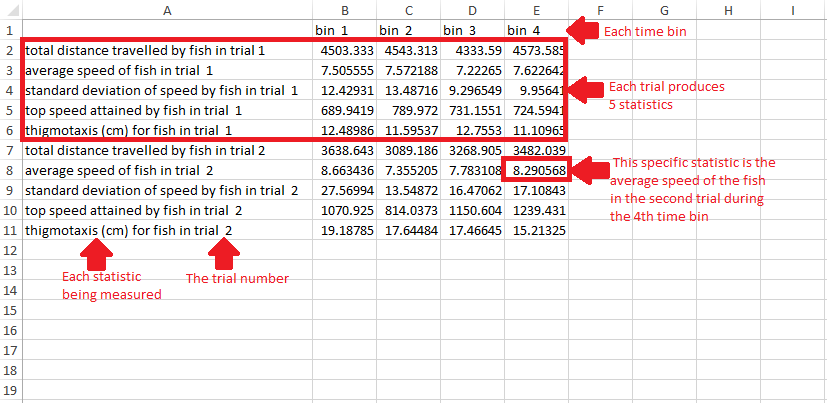
\includegraphics[width=150mm]{image9.png}
\caption{Annotated Output From a File}
\label{overflow}
\end{figure}

\end{document}